%% The following is a directive for TeXShop to indicate the main file
%%!TEX root = diss.tex

\chapter{Including Geological Maps in Model Objective Functions }
\label{ch:GIFtools}
%
%\begin{epigraph}
%
%\end{epigraph}
%
%As Far I as I can tell This section should organized by data type as well.
%
%\section{Forms of A Priori Information}
%\label{sec:Forms of A Priori Information}
%
%\subsection{Bore Hole Data and the Use of Koenigsberger Ratios to Correct Bore Hole Susceptibility Measurements}
%\label{sec: Bore Hole Data}
%
%
%I think there is some use in describing how GIFtools does it now. Much of this work was done in \cite{williams2008geologically}. Mostly what I have done is the inclusion of lithologies and the use of Koenigsberger
%	
%\subsection{Surface Sample Data}
%\label{sec: Surface Sample Data}
%
%Again \cite{williams2008geologically} did much of this. I think the Surface Samples will be primary use in proving physical properties for the map in El Poma
%
%
%\subsection{Geological Maps}
%\label{sec: Geological Maps}

It is often the case that geological information is provided in the form of geological maps in either cross section or plan view. Such maps are particularly useful since they provide a great deal of information over their entire surface. Cross sections can provide information at depth and constrain a whole region often within the center of a target of interest. Plan view maps do not provide information at depth, but they do constrain the entire surface of region being inverted.  Constraining the surface of an inversion is of interest since the sensitivity of the data to the top cells is particularly high which can lead to artifacts on the surface. For the next section the plan view model is from the El Poma case study and the cross section model is from TKC, specifically the map from \citep{harder2006geology}

Below in point form is the method I use to incorporate a pixel map

\section{Preprocessing Images}
\label{sec:Preprocessing}

 (for the purposes of building a geological model the regions on the map have been replaced with solid colours)

\section{Loading Images into GIFtools}
\label{sec:Load Images into GIFtools}

\begin{itemize}
\item load image into the GIFtools format (\autoref{fig:importPlanGui})
\begin{itemize}
	\item determine image format
	\item load image using MATLAB utilities
	\item convert image into .png style representation for faster computation
	\item using .twf file (world file) assign location and spacial resolution to the image
	\item assign a legend assigning pixel RGB values to geological unit
	\item assign topography (either number or GIFtools TOPOdata item) for visualization
	\begin{itemize}
		\item In the case of a cross section image, instead of topography, information for the location of the cross section in 3D or 2D space is required (\autoref{fig:importCrossGui})
	\end{itemize}
\end{itemize}
\end{itemize}
\begin{figure} [h]
    \centering
    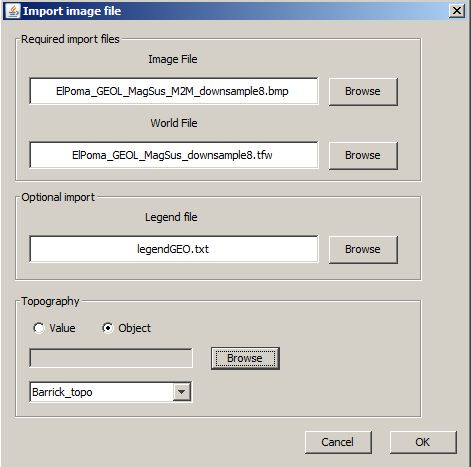
\includegraphics[width=0.5\textwidth]{images/MaptoModel/importPlan.PNG}
    \caption{GUI for importing plan view image }
    \label{fig:importPlanGui}
\end{figure}
\begin{figure} [h]
    \centering
    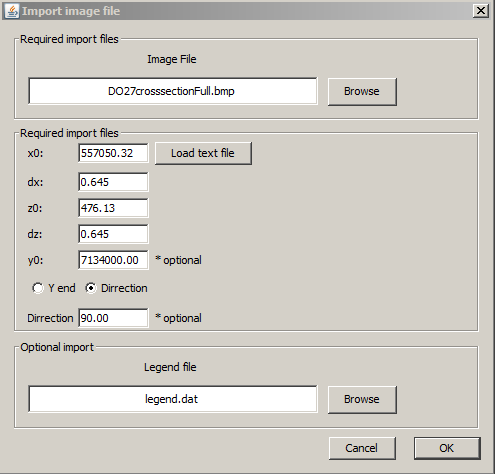
\includegraphics[width=0.5\textwidth]{images/MaptoModel/importCross.PNG}
    \caption{GUI for importing cross section image }
    \label{fig:importCrossGui}
\end{figure}
Storing a map as a GIFtools object allows its use in several ways. Notably it allows the integration of the map with models and data, allowing figures overlaying the map and data or model and allowing interpretation of the data or model with direct reference to the map (\autoref{fig:mapData}).
\begin{figure} [h]
    \centering
    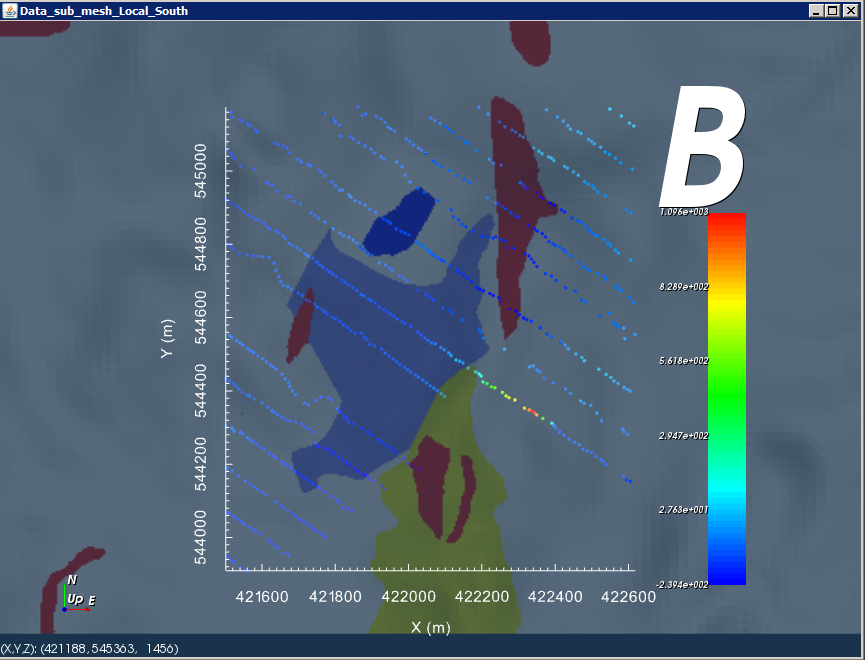
\includegraphics[width=0.5\textwidth]{images/MaptoModel/mapData.PNG}
    \caption{Example of magnetics data being viewed with a map overlaid }
    \label{fig:mapData}
\end{figure}



\section{Creating a Pixel Map Legend}
\label{sec:Create Pixel Map Legend}

Continuing on in the process of making a geological constraint
\begin{itemize}
\item Find the geological unit represented of each pixel
\begin{itemize}
	\item In the .png style format as stored in MATLAB, an image consists of an ``image'' field, a matrix of integers, and a ``map'' field, which maps the image matrix to RBG value triplets
	\item Each RGB triplet is compared to the legend that was provided when the image was loaded. A map field entry is considered to represent a geological unit if all three components of the RGB triplet are within a provided tolerance of any entry in the legend
	\item Now that we have a relation of entries in the map field to geological units in the legend, we can assign a geological unit to each pixel in the original image simply by applying the new geological map to the image field.
\end{itemize}
\end{itemize}

\section{Making a Geology Model from Map}
\label{sec:Make Geology Model from Map}

\subsection{Plan View}
\label{subsec:Make Geology Model from Map Plan View}

\begin{itemize}
\item provide active model	
\begin{itemize}
	\item this simultaneously provides a discretized topography for the map to lay along and also a mesh (\ac{GIF} 3D tensor or OcTree) 
\end{itemize}
\item provide some form of depth information
\begin{itemize}
	\item Thickness, a certain amount of depth below topography at each point will be assigned the geological unit at each 
	\item Depth, the map will be used to assign a geological unit down to a fixed depth across the while model
	\item Surface, if you provide another surface below topography the cells between topography and the other surface will be assigned
\end{itemize}

\item crop all pixels that extend outside of the mesh or that represent the background geological unit
\begin{itemize}
	\item the cropping greatly speeds up the process and makes it require much less computer memory
	\item furthermore, in the event of a mistake with coordinates the process ends almost instantly as there are few pixels to process
\end{itemize}
\item Finally the geological model is created
\begin{itemize}
	\item We determine which cell of the mesh each pixel is in, including those cells below each pixel to account for thickness
	\item each cell is assigned a geological unit based on the mode of the geological values of each pixel
	\begin{itemize}
	\item The mode is used since each cell will be a particular unit. Since the property being mapped onto each cell is a geological unit, interpolation between the units will not provide the desired result
	\end{itemize}
	\item the geology definition which will allow the assignment of physical properties to each geological unit
\end{itemize}
\end{itemize}
\begin{figure} [h]
    \centering
    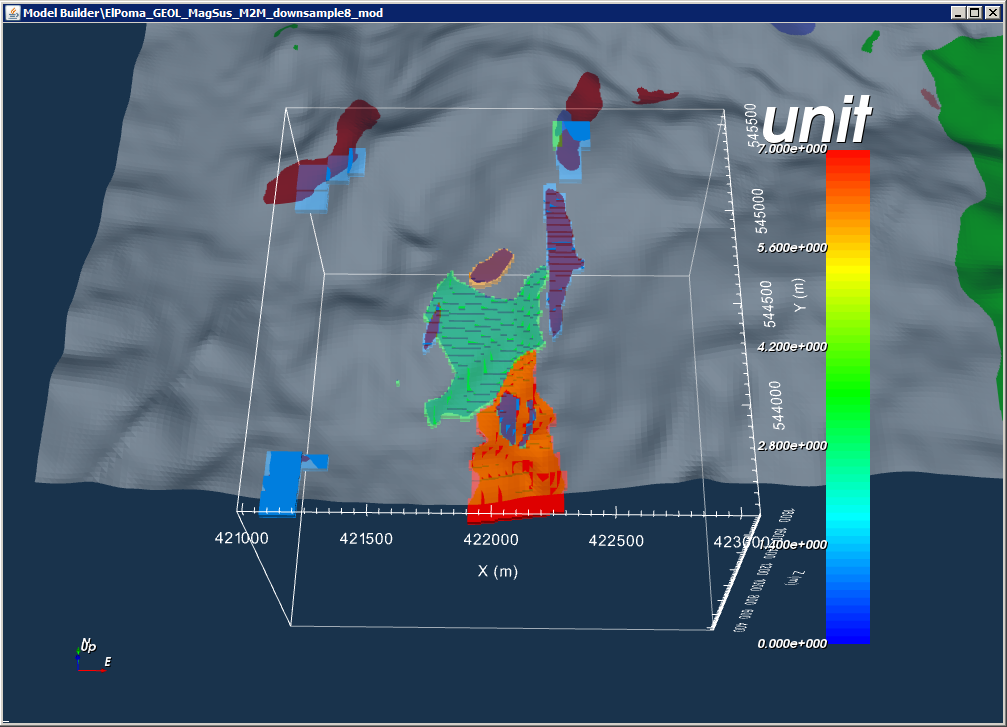
\includegraphics[width=0.5\textwidth]{images/MaptoModel/mapModelPlan.PNG}
    \caption{Example of a geology model created from a map with the map overlaid}
    \label{fig:mapModelPlan}
\end{figure}

\subsection{Cross Section}
\label{subsec:Make Geology Model from Map Cross Section}

The cross section case follows much the same procedure with a few exceptions. An imported cross section map is shown overlaid on a 2D mesh in \autoref{fig:mapMeshCross}. Notably no parameter for the vertical extent is needed. The other notable exception is that mesh that is used is a \ac{GIF} 2D mesh. The result is shown in \autoref{fig:mapModelCross}.  

A 2D Geology model can be used to create constraints for a 2D inversion, it can also be used to add constraints to a 3D inversion as well. After the 2D geology model is created from the cross section map, it can be inserted into a 3D mesh (\ac{GIF} 3D tensor or OcTree) given a starting and ending position or a starting position and a direction \autoref{fig:add2Dto3D},\autoref{fig:mapModelCross3D}.

\begin{figure} [h]
    \centering
    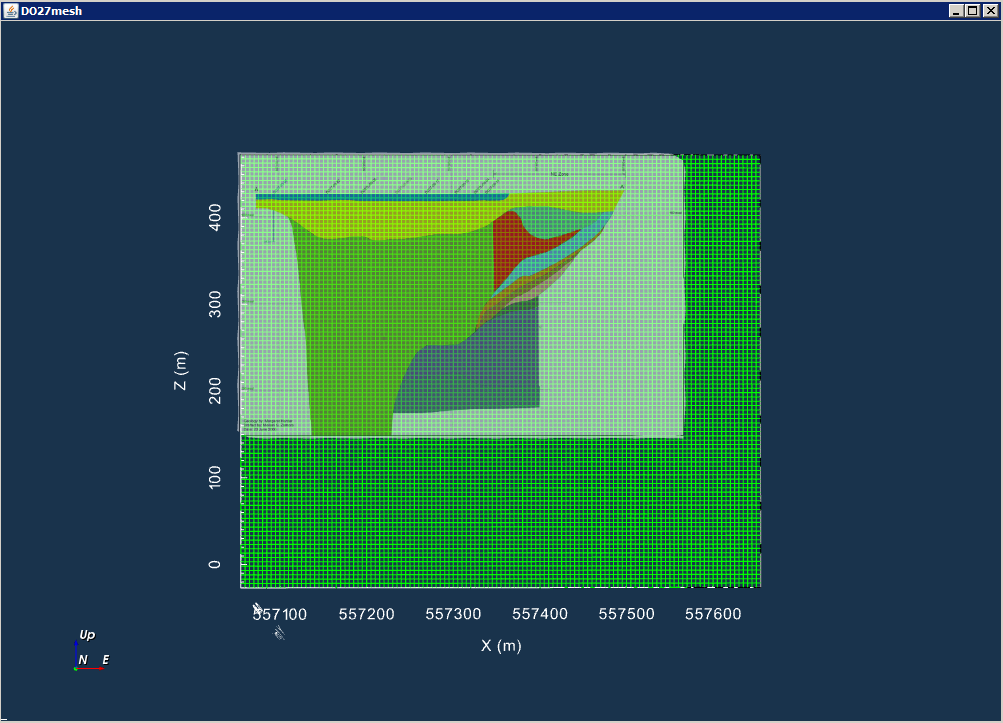
\includegraphics[width=0.5\textwidth]{images/MaptoModel/mapMeshCross.PNG}
    \caption{Example of a 2D mesh with the map overlaid}
    \label{fig:mapMeshCross}
\end{figure}
\begin{figure} [h]
    \centering
    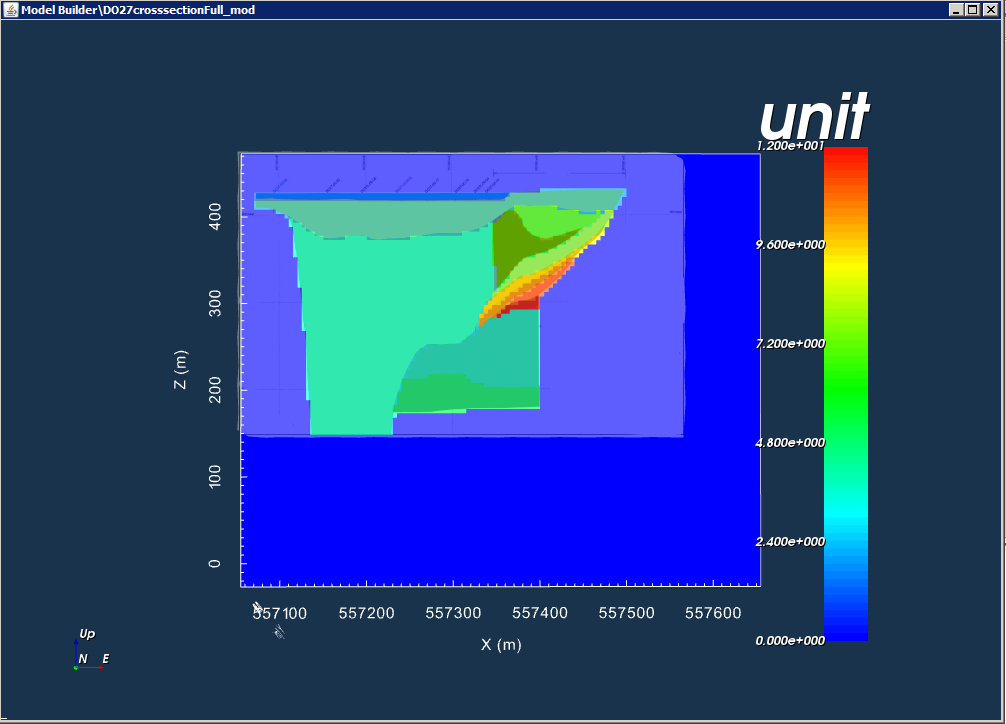
\includegraphics[width=0.5\textwidth]{images/MaptoModel/mapModelCross.PNG}
    \caption{Example of a 2D geology model created from a cross section map with the map overlaid}
    \label{fig:mapModelCross}
\end{figure}
\begin{figure} [h]
    \centering
    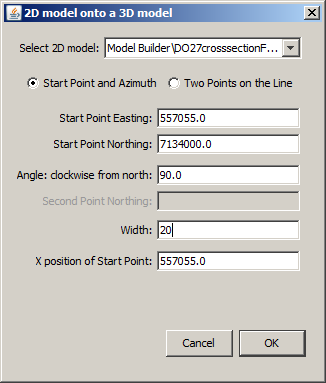
\includegraphics[width=0.5\textwidth]{images/MaptoModel/add2Dto3D.PNG}
    \caption{GUI for adding a 2D model to a 3D model}
    \label{fig:add2Dto3D}
\end{figure}
\begin{figure} [h]
    \centering
    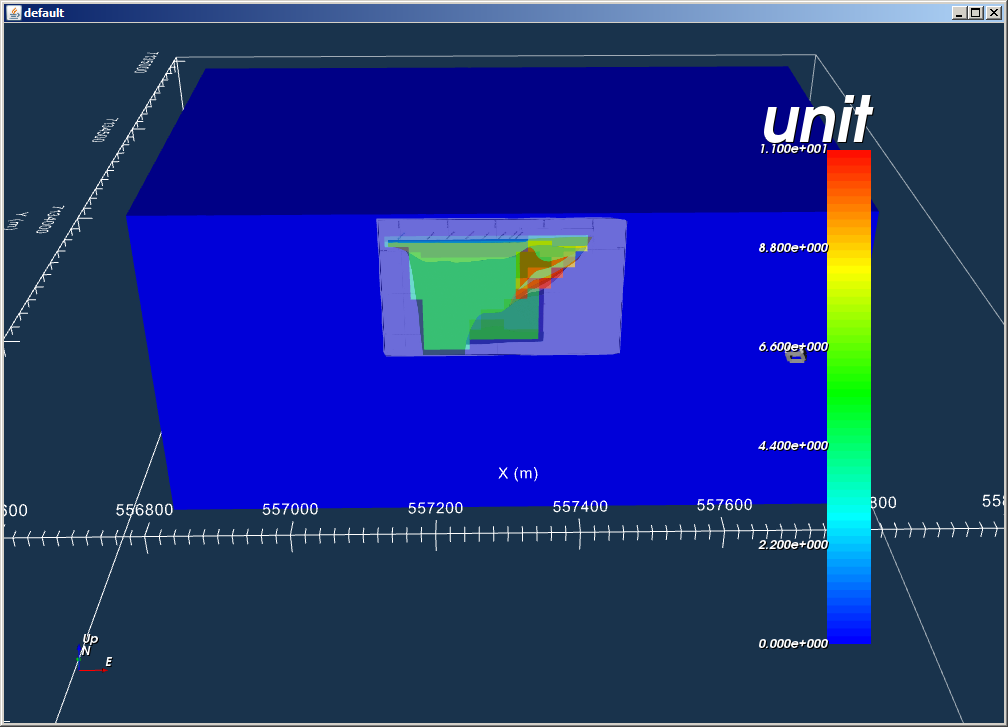
\includegraphics[width=0.5\textwidth]{images/MaptoModel/mapModelCross3D.PNG}
    \caption{Example of a 2D geology inserted into a 3D model with the map overlaid}
    \label{fig:mapModelCross3D}
\end{figure}
\FloatBarrier
\section{Making Constraints for an Inversion}
\label{sec:Making Constraints for and Inversion}

The model that has been created is a geology model. That is, a model in which each cell represents a given geological unit. To be able to convert this model into a constraint for a geophysical inversion some link between between the geology and the petrophysics needs to be provided. 

The link is stored in what is called a geology definition. In GIFtools this takes the form of a lookup table that contains information of a particular geological unit's property, lower and upper bounds, and optionally the smallness weight associated with each unit. 

Using the geology definition we can convert a geology model that has information about the spacial distribution of geological units but not of their physical properties into constraints that are usable by an inversion. In the figures below the geological definition came from surface measurements of magnetic susceptibility within each geological unit. \autoref{fig:geoDefPlan} is an example of a geology definition in the GIFtools GUI.
\begin{figure} [h]
    \centering
    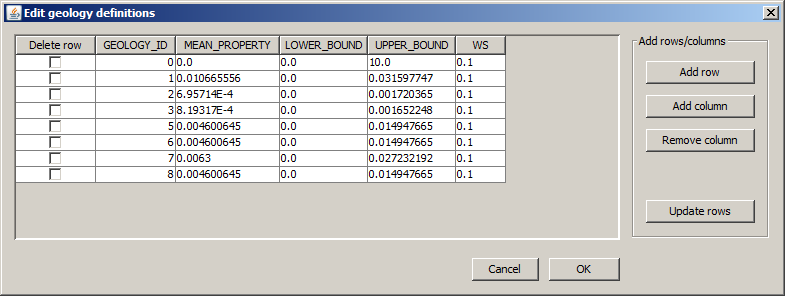
\includegraphics[width=0.8\textwidth]{images/MaptoModel/geoDefPlan.PNG}
    \caption{Example of a geological definition as displayed in the GIFtools GUI}
    \label{fig:geoDefPlan}
\end{figure}

Once the geology definition is provided, we can use the Combine Model Dialog (\autoref{fig:combineModelRef}) in Model Builder to create a reference model and bounds. 
\begin{figure} [h]
    \centering
    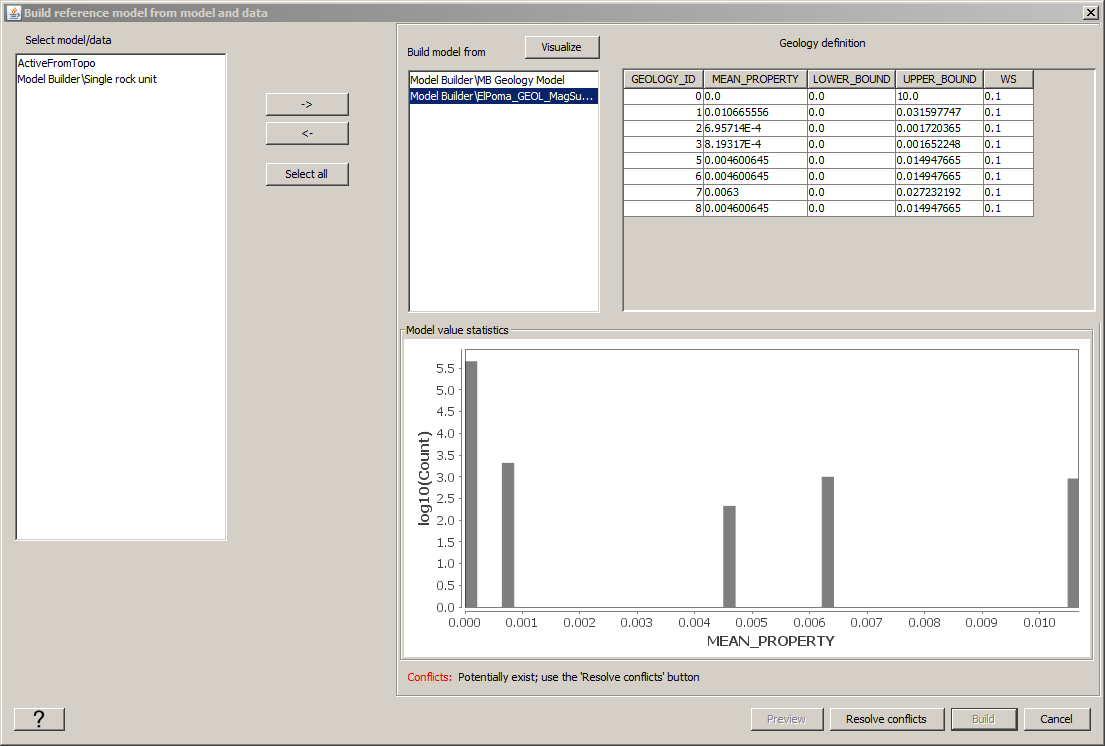
\includegraphics[width=0.8\textwidth]{images/MaptoModel/combineModelRef.PNG}
    \caption{Example of a typical combine model dialog for a reference model}
    \label{fig:combineModelRef}
\end{figure}
In this case the resolution of conflicts is trivial as there is a single source of information. Less trivial examples of the creation of reference models and bounds will be discussed later. The resulting reference model is shown in \autoref{fig:mapRefModPlan}.
\begin{figure} [h]
    \centering
    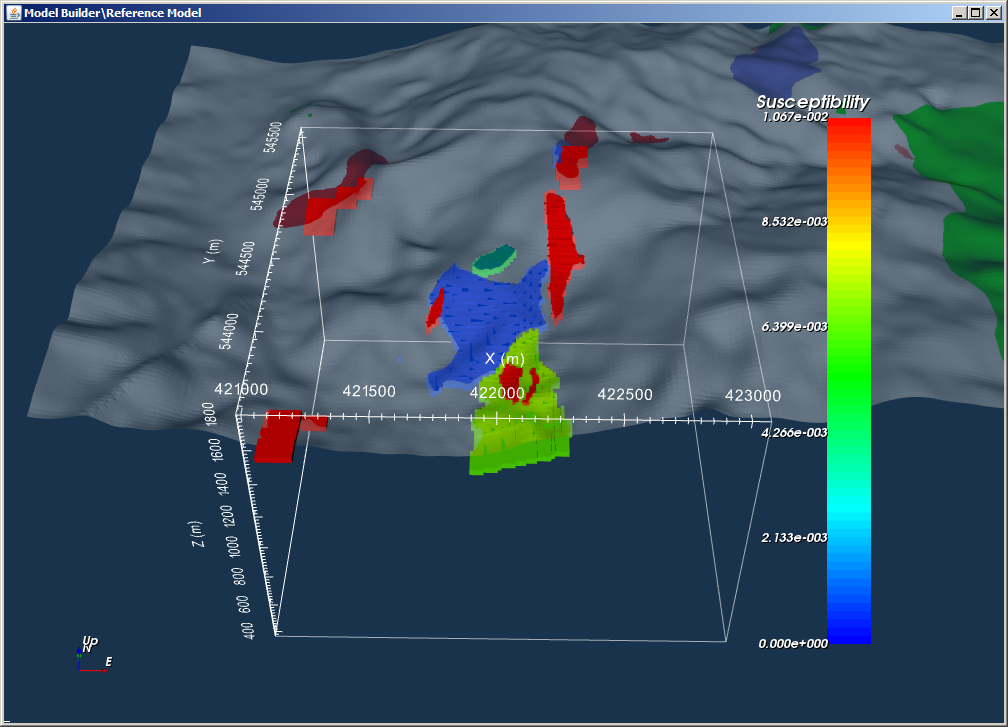
\includegraphics[width=0.8\textwidth]{images/MaptoModel/mapRefModPlan.PNG}
    \caption{Example of a reference model created from a geological map}
    \label{fig:mapRefModPlan}
\end{figure}

\section{Inputing Fault information from Geological Maps}
\label{sec:Inputing Fault information from Geological Maps}

Another piece of information that can be in geological maps are fault locations. Again in the context of El Poma the map provided a whole complex of thrust faults as shown in the un-doctored map in \autoref{fig:ElPoma_GEOL_MagSus}
\begin{figure} [h]
    \centering
    \frame{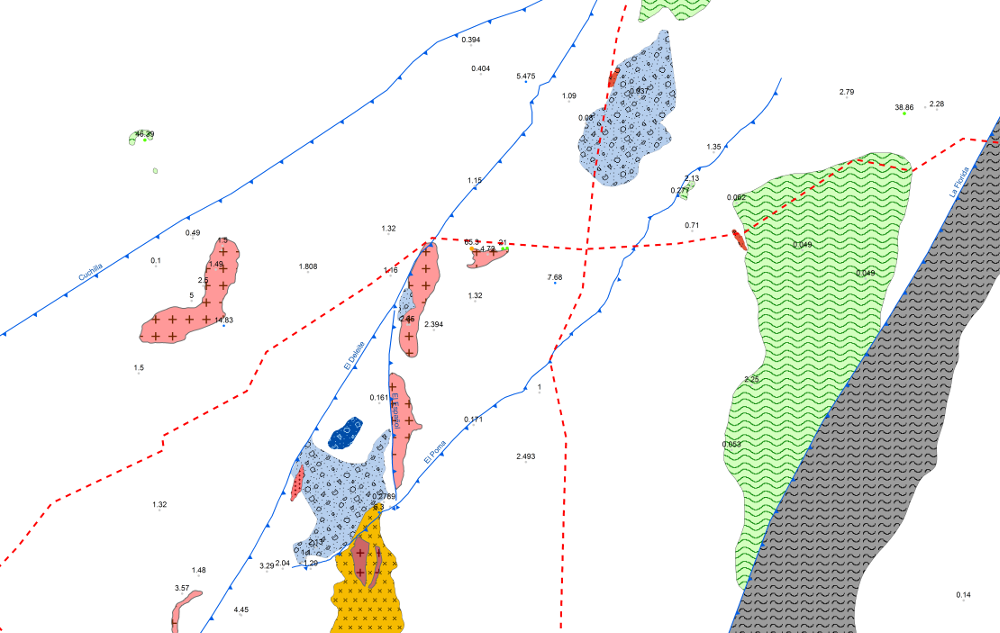
\includegraphics[width=0.8\textwidth]{images/Faults/ElPoma_GEOL_MagSus.png}}
    \caption{The El Poma map with fault lines (blue lines with barbs) included}
    \label{fig:ElPoma_GEOL_MagSus}
\end{figure}
\FloatBarrier
The method used to insert faults into an inversion is as follows

\begin{itemize}
\item Determine the end points of the fault.
\begin{itemize}
	\item GIFtools makes this easy by reporting the location of the cursor in the data viewer allowing you to find the location (including elevation) of a point along the fault
\end{itemize}
\item Using the locations provided create a box of a desired thickness (default value is based on the core mesh size) that includes the ends points of the fault and dips in the desired direction
\item faces within this box are assigned a new value that is provided in the GUI \autoref{fig:makeFaultGUI}
\end{itemize}

\begin{figure} [h]
    \centering
    \frame{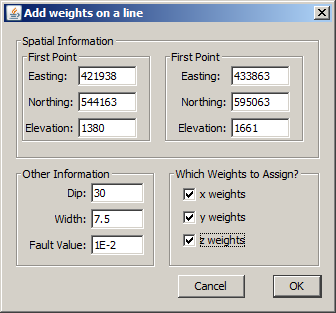
\includegraphics[width=0.5\textwidth]{images/Faults/makeFaultGUI.png}}
    \caption{The GUI for the creation of fault weights}
    \label{fig:makeFaultGUI}
\end{figure}

This process can be done multiple times to create non-trivial fault complexes as shown in \autoref{fig:faults}

\begin{figure} [h]
    \centering
    \frame{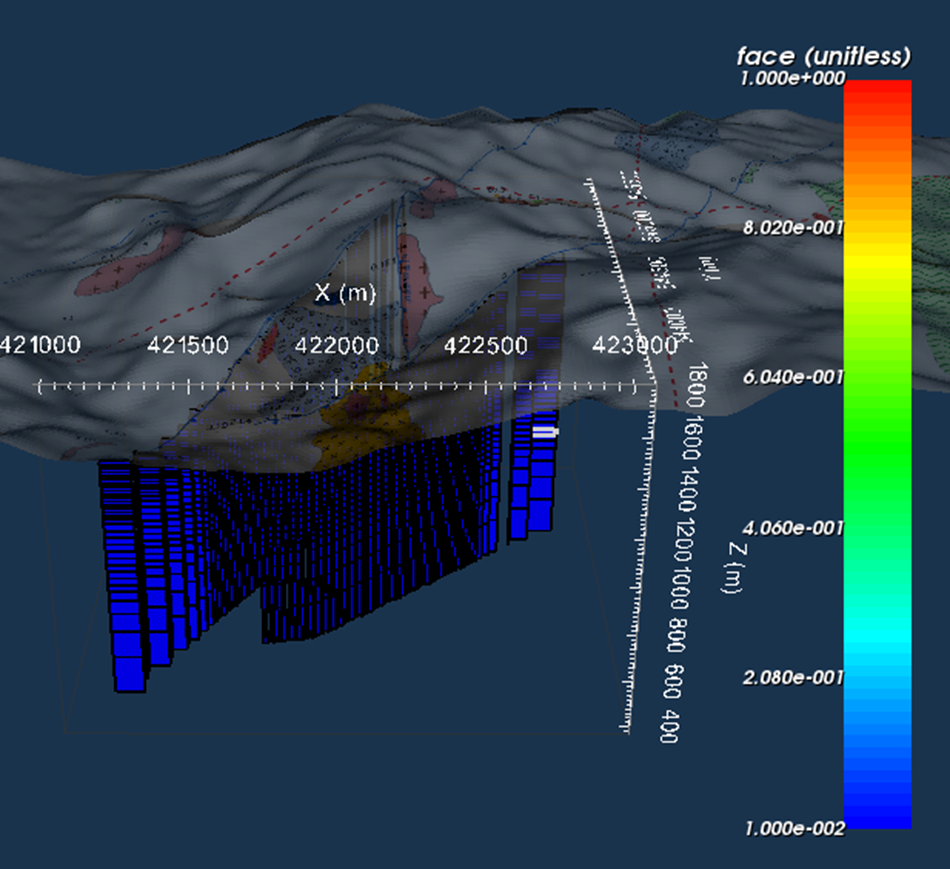
\includegraphics[width=0.5\textwidth]{images/Faults/faults.png}}
    \caption{An example of fault weights that can be created with GIFtools}
    \label{fig:faults}
\end{figure}
\FloatBarrier

In this section I have shown the creation of constraints that are compatiple with \ac{GIF} inversion codes. I have created these constraints from multiple types of map (Cross Section and Plan View) and have used different pieces of information from these maps (geological units and fault locations).



%\section{Using Multiple Data Types, with Clustering}
%\label{sec:Using Multiple Data Types, with Clustering}
%
%There is interesting things to discuss in the storing of multiple inversion in GIFtools, and in the use of clustering algorythms used and then ability to take geological models and make reference models and non-trivial face weighting.

\endinput

Any text after an \endinput is ignored.
You could put scraps here or things in progress.
